% Notes:
%
% Can we prove in a line or two that the inverse problem is stable by arguing that the function is bijective and closed therefore a homeomorphism?
% Should we mention the notion of Grassmannian manifolds and that Theta is a metric on this space?
% Change robustness to stability?
%
\documentclass[journal, twocolumn]{IEEEtran}

% *** MATH PACKAGES ***
\usepackage{amsmath, amssymb, amsthm} 
\newtheorem{theorem}{Theorem}
\newtheorem{lemma}{Lemma}
\newtheorem{conjecture}{Conjecture}
\newtheorem{problem}{Problem}
\newtheorem{question}{Question}
\newtheorem{proposition}{Proposition}
\newtheorem{definition}{Definition}
\newtheorem{corollary}{Corollary}
\newtheorem{remark}{Remark}
\newtheorem{example}{Example}


\usepackage[pdftex]{graphicx}

% *** ALIGNMENT PACKAGES ***
\usepackage{array}

% correct bad hyphenation here
%\hyphenation{op-tical net-works semi-conduc-tor}

\begin{document}

\title{Sparse Coding is Stable}

\author{Charles~J.~Garfinkle and Christopher~J.~Hillar \\
Redwood Center for Theoretical Neuroscience, Berkeley, CA, USA
\thanks{%Redwood Center for Theoretical Neuroscience, Berkeley, CA, USA.  % ; e-mails: cjg@berkeley.edu, chillar@msri.org.  
Support was provided, in part, by National Science Foundation grants IIS-1219212 (CH), IIS-1219199 (CG), and a SAMSI Working Group (CH, CG).}}


\maketitle

\begin{abstract}
Sparse coding has exposed underlying structure in many kinds of natural data.  However, given the multitude of algorithms implementing this strategy, claims of ``true" latent discovery require the backing of universal theorems guaranteeing statistical consistency.  Here, we prove that for almost all diverse enough datasets generated under this model, sparse coding to within a constant multiple of measurement noise uniquely identifies original codes and dictionary up to uniform permutation/scaling ambiguities and commensurate error.  Applications are given to smoothed analysis, neuroscience, and engineering.
\end{abstract}

\begin{IEEEkeywords}
Bilinear inverse problem, matrix factorization, identifiability, dictionary learning, sparse coding, compressed sensing, blind source separation, sparse component analysis
\end{IEEEkeywords}

%===================================
% 			INTRODUCTION
%===================================

% Mention application to data compression
% Also I should translate epsilon into angle, i.e. the norm in the matrix space into the metric in the space of subspaces.
\section{Introduction}
\IEEEPARstart{E}{ver} since sparse coding of natural images reproduced response properties of neurons in mammalian primary visual cortex \cite{Olshausen96}, learning sparse representations of vector-valued data has become an important component of many signal processing and machine learning applications (see \cite{Zhang15} for a comprehensive review). In the \textit{sparse coding} model, each vector in a dataset $Z = \{\mathbf{z}_1, \ldots, \mathbf{z}_N\} \subset \mathbb{R}^n$ is approximated as a linear combination of $k$ vectors drawn from a learned \emph{dictionary} $\mathcal{A} \subset \mathbb{R}^n$, where $k \ll n \leq m:= |\mathcal{A}| \ll N$. 

Many algorithms have been designed to infer the underlying parameters of this model, and it is tempting to accept their output as approximating ``ground truth" (e.g., animal position on a linear track \cite{Agarwal14}) when it exists. However, it is possible that several qualitatively different solutions are nonetheless consistent with the data. It is therefore important to determine algorithm-independent conditions guaranteeing when the sparse representation of a dataset is uniquely identifiable up to natural symmetries and also stable with respect to noise. 
%a dictionary $\mathcal{A}$ of a given size can be uniquely identified up to natural symmetries from a dataset $Y$ and when each datum, in turn, has a unique sparse decomposition into elements of this dictionary. 

The significant finding of this work is that any dictionary satisfying the spark condition from compressed sensing (CS) is uniquely identifiable from enough sparse noisy linear combinations of its elements up to an error linear in the noise (Thm.~\ref{DeterministicUniquenessTheorem}).
%We note that this is a necessary condition if the dataset $Y$ could in principle include data generated as in \eqref{LinearModel} from any given $k$-sparse vector $\mathbf{x} \in \mathbb{R}^m$. 
% [ *** Can we motivate more necessary conditions using theorems of Li15, too? Thm.~2.8. *** ] 
%We also characterize the stability of these solutions with respect to noise, an essential consideration as measurements are inevitably rendered uncertain by various sources of error.
The explicit criteria under which this result holds can serve as a theoretical tool in the analysis of sparse coding routines, some of which now provably converge to a global solution when it exists (see \cite[Sec.~I-E]{Sun16} for a brief discussion of the state-of-the-art in these algorithms). 

%Several related problems seem to fall under the umbrella term of sparse coding (also ``dictionary learning" or ``sparse component analysis") \cite{Zhang15}. We consider the following formulation of sparse coding (also ``dictionary learning" or ``sparse component analysis"), which we believe best represents the original motivating philosophy. 
We consider the following formulation of the sparse coding problem (also ``dictionary learning" or ``sparse component analysis"). Fix a dictionary represented as the columns $A_j$ of a matrix $A \in \mathbb R^{n \times m}$. Suppose  $Z$ consists of measurements:
\begin{align}\label{LinearModel}
\mathbf{z} = A\mathbf{a} + \mathbf{n},
\end{align}
for $k$-\emph{sparse} $\mathbf{a} \in \mathbb{R}^m$ having at most $k$ nonzero entries, and \emph{noise} $\mathbf{n} \in \mathbb{R}^n$, with $|\mathbf{n}|_2 \leq \varepsilon$. The noise represents our combined worst-case uncertainty in  measuring $\mathbf{y} = A\mathbf{a}$.
%; if these uncertainties are all bounded then, since they sum linearly, the resulting total is also bounded, i.e. we suppose for all data in $Y$ that $|\mathbf{n}|_2 \leq \varepsilon$ for some $\varepsilon \geq 0$. 

\begin{problem}[Sparse Coding]\label{InverseProblem}
Find $B \in \mathbb{R}^{n \times m}$ and $k$-sparse $\mathbf{b}_1, \ldots, \mathbf{b}_N \in \mathbb{R}^m$ such that $|\mathbf{z}_i - B\mathbf{b}_i|_2 \leq \varepsilon$ for $i = 1, \ldots, N$.
\end{problem}

Any solution to this problem admits an inherent permutation-scaling ambiguity, since $B = AD^{-1}P^{\top}$ and $k$-sparse $\mathbf{b}_i = PD\mathbf{a}_i$ also give the same reconstruction error for any permutation matrix $P \in \mathbb{R}^{m \times m}$ and invertible diagonal matrix $D \in \mathbb{R}^{m \times m}$. Previous works \cite{li2004analysis, Georgiev05, Aharon06, Hillar15}  addressing the case $\varepsilon = 0$ have proved that the solutions are indeed unique up to this inherent ambiguity for sufficiently large $N$ provided the matrix $A$ satisfies the \textit{spark condition}:
\begin{align}\label{SparkCondition}
A\mathbf{x}_1 = A\mathbf{x}_2 \implies \mathbf{x}_1 = \mathbf{x}_2,\indent \text{for all $k$-sparse } \mathbf{x}_1, \mathbf{x}_2,
\end{align}
%
which is evidently a necessary condition if the $\mathbf{a}_i$ are known only to be $k$-sparse. Matrices of the form $PD$ thus form the \emph{ambiguity transformation group} inherent to the noiseless problem when $N$ is large enough \cite{Li15}. We introduce the following terminology to handle the general case.

% no need for this in this paper -- a bit confusing to throw in 
%When they exist, solutions to Problem \ref{InverseProblem} will be found by solving:
%\begin{align*}
%\min_{B, \, \mathbf{b}_i} \  \max_{i \in [N]} |\mathbf{b}_i|_0 \text{ s.t. } |\mathbf{y}_i - B\mathbf{b}_i|_2 \leq \varepsilon \text{ for $i = 1, \ldots, N$}.
%\end{align*}

% Actually the main finding are the specific bounds. Necessary conditions can be derived from the BIP paper...
%This is because any dictionary $\mathcal{D}$ generates infinitely many distinct but equally expressive dictionaries by scaling the elements of $\mathcal{D}$ by nonzero factors; hence, the data in $Y$ could have been generated by any one of these alternate dictionaries. This scaling ambiguity is inherent to all bilinear inverse problems \cite{Choudhary14}.  An additional permutation ambiguity derives from the arbitrary ordering mapping elem`ents of $\mathcal{D}$ to columns of $A$.  
%Equivalently, one could interpret the dictionary learning problem as one of identifying a set of elements in a space which equates all points in $\mathbb{R}^{n} \setminus \{\mathbf{0}\}$ which are nonzero scalings of one another (i.e. the set of lines through the origin), in which case the uniqueness of a solution retains its usual meaning. 
% Pretty version: BIPs should all be rephrased in projective space rather than redefine uniqueness?
% yes:  S_m \times \mathbb (P^1(\mathbb R))^m
%If $\varepsilon = 0$, though, then solutions to Problem \ref{InverseProblem} are unique up to this permutation-scaling ambiguity  

\begin{definition}\label{Uniqueness}
We say a set of vectors $Y = \{ \mathbf{y}_1, \ldots, \mathbf{y}_N\}$ has a \textbf{$k$-sparse representation in $\mathbb{R}^m$} when for some $A \in \mathbb{R}^{n \times m}$ and $k$-sparse $\mathbf{a}_1, \ldots, \mathbf{a}_N \in \mathbb{R}^m$, we have $\mathbf{y}_i = A\mathbf{a}_i$ for $i = 1, \ldots, N$. This representation is \textbf{stable} if for every $\delta_1, \delta_2 \geq 0$, there exists $\varepsilon \geq 0$ (with $\varepsilon > 0$ when  $\delta_1, \delta_2 > 0$) such that if a matrix $B \in \mathbb{R}^{n \times m}$ and $k$-sparse $\mathbf{b}_1, \ldots, \mathbf{b}_N \in \mathbb{R}^m$ 
solve Problem~\ref{InverseProblem},
%satisfy:
%\begin{align}\label{y-Bb}
%|\mathbf{y}_i - B\mathbf{b}_i|_2 \leq \varepsilon,\indent \text{for } i = 1, \ldots, N,
%\end{align}
there is a permutation matrix $P \in \mathbb{R}^{m \times m}$ and invertible diagonal matrix $D \in \mathbb{R}^{m \times m}$ such that for all $i,j$:
\begin{align}\label{def1}
|A_j - (BPD)_j|_2 \leq \delta_1 \ \ \text{and} \ \ |\mathbf{a}_i - D^{-1}P^{\top}\mathbf{b}_i|_1 \leq \delta_2.
\end{align}
\end{definition}

\begin{question}\label{DUTproblem}
When does a dataset $Y = \{\mathbf{y}_1, \ldots, \mathbf{y}_N \} \subset \mathbb{R}^n$ have a stable $k$-sparse representation in $\mathbb{R}^m$?
\end{question}

It is not hard to see how an answer to Question \ref{DUTproblem} informs the interpretation of solutions to Problem \ref{InverseProblem}. Let $Z$ be a generated as in \eqref{LinearModel}, where $A$ and the $\mathbf{a}_i$ are such that the  noiseless measurements $\mathbf{y}_i = A\mathbf{a}_i$ have a stable $k$-sparse representation in $\mathbb{R}^m$. Fix $\delta_1, \delta_2 \geq 0$, the desired accuracy in uniqueness, and let $\varepsilon(\delta_1, \delta_2)$ be as in Def.~\ref{Uniqueness}. 
% there is no triangle inequality, just the exact definition
If $\varepsilon \leq \frac{1}{2}\varepsilon(\delta_1, \delta_2)$, then any solution to Problem~\ref{InverseProblem} necessarily satisfies \eqref{def1} for some $P$, $D$. 
%That is, the dictionary and codes are uniquely determined to within $\delta_1$ and $\delta_2$, respectively, up to the inherent permutation-scaling ambiguity %and an error commensurate with noise.

Thm.~\ref{DeterministicUniquenessTheorem}, stated in Sec.~\ref{Results}, provides an answer to Question \ref{DUTproblem} from which we then derive an explicit form for $\varepsilon(\delta_1, \delta_2)$.  We also provide a probabilistic version of the result (Thm.~\ref{ProbabilisticTheorem}) and an extension to the case when only an upper bound on the dimensionality of the sparse codes (i.e., the number of columns in the generating dictionary) is known (Thm.~\ref{DeterministicUniquenessTheorem2}). 

We prove Thm.~\ref{DeterministicUniquenessTheorem} in Sec.~\ref{DUT} after listing some additional definitions and key lemmas required for the proof, including our main tool from combinatorial matrix analysis (Lem.~\ref{MainLemma}). All other proofs are relegated to the supplementary materials. The final section contains a discussion of potential applications.

%In Section \ref{mleqm}, we state another extension of this result (Thm.~\ref{DeterministicUniquenessTheorem2}) to the case where only an upper bound on the dimensionality of the sparse codes (or, equivalently, the number of columns in the generating dictionary) is known. 
%In Section \ref{PUT}, we state Thm.~\ref{ProbabilisticTheorem}, our probabilistic version of Thm.~\ref{DeterministicUniquenessTheorem}. 
%Supplementary materials contain proofs of Cor.~\ref{DeterministicUniquenessCorollary}, Thms.~\ref{DeterministicUniquenessTheorem2}~and~\ref{ProbabilisticTheorem} and our main tool, Lem.~\ref{MainLemma}.

\section{Results}\label{Results}

Before precisely stating our results, we explain how the spark condition \eqref{SparkCondition} relates to the \emph{lower bound} \cite{Grcar10} of $A$, written $L(A)$, which is the largest number $\alpha$ such that $|A\mathbf{x}|_2 \geq \alpha|\mathbf{x}|_2$ for all $\mathbf{x} \in \mathbb{R}^m$. By compactness, every injective linear map has a nonzero lower bound; hence, if $A$ satisfies \eqref{SparkCondition} then every submatrix formed from $2k$ of its columns or less has a nonzero lower bound. We therefore define the following domain-restricted lower bound of $A$:
\begin{align*}
L_k(A) := \max \{ \alpha : |A\mathbf{x}|_2 \geq \alpha|\mathbf{x}|_2 \text{ for all $k$-sparse } \mathbf{x} \in \mathbb{R}^m\}.
\end{align*} 
Clearly, $L_k(A) \geq L_{k'}(A)$ whenever $k < k'$, and for any $A$ satisfying \eqref{SparkCondition} we have $L_{k'}(A) > 0$ for all $k' \leq 2k$. 

A \textit{cyclic order} on $[m] := \{1, \ldots,m\}$ is an arrangement of $[m]$ in a circular necklace, and an \textit{interval} in the order is any subset of contiguous elements. A vector $\mathbf{a} \in \mathbb{R}^m$ is said to be \emph{supported} on $S \subseteq [m]$ when $\mathbf{a} \in \text{Span}\{ \{\mathbf{e}_i\}_{i\in S}\}$, where $\mathbf{e}_i$ are the standard basis vectors.  Also, recall that $M_j$ denotes the $j$th column of a matrix $M$. The following is our main result.

%=== STATEMENT OF DETERMINISTIC UNIQUENESS THEOREM ===%
\begin{theorem}\label{DeterministicUniquenessTheorem}
Fix $n, m$, and $k < m$. If $A \in \mathbb{R}^{n \times m}$ satisfies spark condition \eqref{SparkCondition} and $k$-sparse \mbox{$\mathbf{a}_1, \ldots, \mathbf{a}_N \in \mathbb{R}^m$} are such that for every interval of length $k$ in some cyclic order on $[m]$ there are at least \mbox{$(k-1){m \choose k}+1$} vectors $\mathbf{a}_i$ in general linear position (i.e., any $k$ of them are linearly independent) supported there, then $Y = \{A\mathbf{a}_1, \ldots, A\mathbf{a}_N\}$ has a stable $k$-sparse representation in $\mathbb{R}^m$.

Specifically, there exists a constant $C > 0$ for which the following holds for all $\varepsilon < \frac{L_2(A)}{\sqrt{2}}C^{-1}$. If any matrix $B \in \mathbb{R}^{n \times m}$ and $k$-sparse $\mathbf{b}_1, \ldots, \mathbf{b}_N \in \mathbb{R}^m$ are such that \mbox{$|A\mathbf{a}_i - B\mathbf{b}_i|_2 \leq \varepsilon$} for all $i \in [N]$, then for all $j \in [m]$:
\begin{align}\label{Cstable}
|A_j-(BPD)_j|_2 \leq C\varepsilon,
\end{align}
%
for some permutation matrix $P \in \mathbb{R}^{m \times m}$ and invertible diagonal matrix $D \in \mathbb{R}^{m \times m}$.  Moreover, if $\varepsilon < \varepsilon_0 := \frac{L_{2k}(A)}{\sqrt{2k}}C^{-1}$ then $B$ also satisfies the spark condition and for all $i \in [N]$:
\begin{align}\label{b-PDa}
|\mathbf{a}_i - D^{-1}P^{\top}\mathbf{b}_i|_1 &\leq \frac{\varepsilon }{ \varepsilon_0 - \varepsilon} \left( C^{-1}+|\mathbf{a}_i|_1 \right).
\end{align}
\end{theorem}

\begin{remark}
Note that it was not assumed a priori that $B$ satisfy the spark condition. In fact, when $\varepsilon < \varepsilon_0$, we have $L_{2k}(BPD) \geq L_{2k}(A)\left( 1 - \frac{\varepsilon}{\varepsilon_0} \right)$.
\end{remark}


%\begin{figure}[b!]
%\begin{center}
%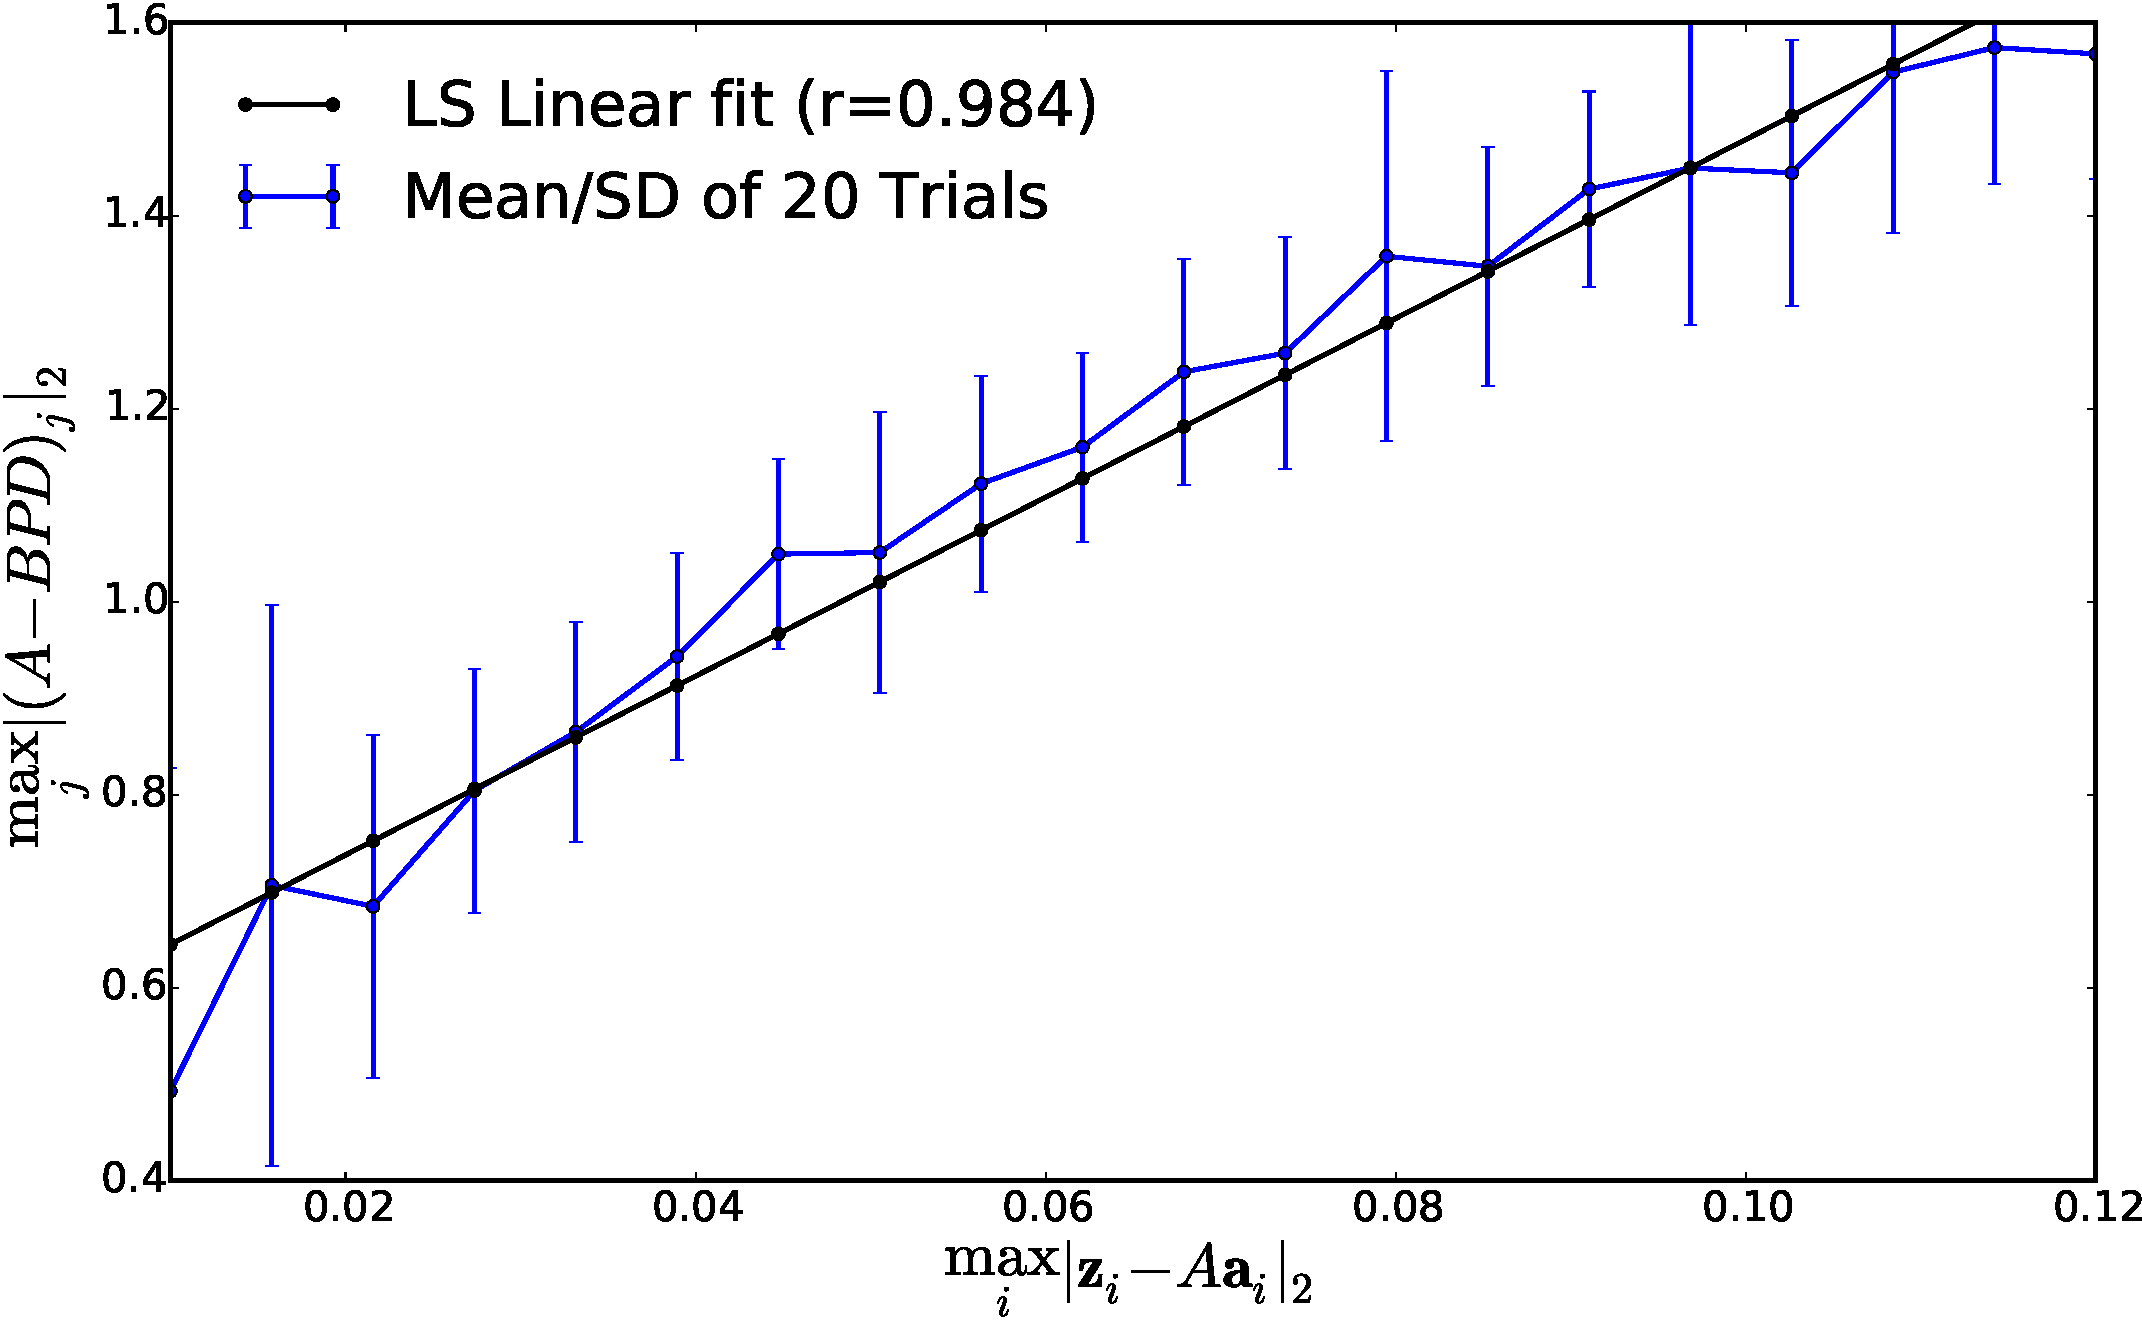
\includegraphics[width=\linewidth]{figs/robust_error.pdf}
%\caption{\textbf{Recovery error vs. noise}.  Fast ICA \cite{hyvarinen1999fast} and noise tolerance.}\label{ica_robust}
%\end{center}
%\end{figure}

% Can we get rid of the k-sparse assumption on b using results from CS?

%\begin{remark}[Support Properties]
%Note that the bound in \eqref{b-PDa} does not immediately entail that $\mathbf{a}_i$ and $D^{-1}P^{-1}\mathbf{b}_i$ share the same support unless $\varepsilon = 0$. If $\varepsilon$ is small enough, however, then it is indeed the case that $\text{supp}(D^{-1}P^{-1}\mathbf{b}_i) \subseteq \text{supp}(\mathbf{a}_i)$. [*** TODO: Is this right? See Donoho paper on L1 stability? ***]
% Kinf of like m' > m scenario
%\end{remark}

%[ *** So inference is stable for small enough error! There is no multiplicity of alternative models that also happen to work. Regression models have a fixed $A$ (i.e. the values of the variables we are regressing on). Here, in this model, we don't specify the $A$, instead we learn what the best regressor variables would be if they existed. And we want to combine regressors for different problems so as to save resources. Thought of all this reading section 8 of the Breiman paper on data models vs. algorithmic models.***]

As an important consequence, for sufficiently small reconstruction error, the original dictionary and codes are determined up to a commensurate error. Specifically, for $\delta_1, \delta_2 \geq 0$, Thm.~\ref{DeterministicUniquenessTheorem} says that \eqref{def1} is implied for any $\varepsilon < \varepsilon_0$ satisfying:
\begin{align*}
\varepsilon \leq \min \left( \delta_1 C^{-1}, \frac{ \delta_2 \varepsilon_0}{\delta_2 + C^{-1} + \max_{i \in [N]} |\mathbf{a}_i|_1} \right).
\end{align*}
The constant $C$ is explicitly defined in \eqref{Cdef}, below. 

\begin{corollary}\label{DeterministicUniquenessCorollary}
Given $n, m$, and $k < m$, there are $N =  m(k-1){m \choose k}+m$ vectors \mbox{$\mathbf{a}_1, \ldots, \mathbf{a}_N \in \mathbb{R}^m$} such that every matrix $A \in \mathbb{R}^{n \times m}$ satisfying \eqref{SparkCondition} generates a set $Y = \{A\mathbf{a}_1, \ldots, A\mathbf{a}_N\}$ with a stable $k$-sparse representation in $\mathbb R^m$.
\end{corollary}

Our proof of Thm.~\ref{DeterministicUniquenessTheorem} in Sec.~\ref{DUT} is a refinement of the arguments in \cite{Hillar15} to handle noise and to reduce the number of required samples from $N=k{m \choose k}^2$ to $N = m(k-1){m \choose k}+m$. 

It is straightforward to provide a probabilistic extension of Thm.~\ref{DeterministicUniquenessTheorem} using the following fact in random matrix theory.  The matrix $A \in \mathbb{R}^{n \times m}$ satisfies \eqref{SparkCondition} with probability $1$
%(or ``high probability" for discrete variables) 
provided:
\begin{align}\label{CScondition}
n \geq \gamma k\log\left(\frac{m}{k}\right),
\end{align}
where $\gamma$ is a positive constant dependent on the particular continuous distribution from which the entries of $A$ are sampled i.i.d. (many ensembles suffice, e.g. \cite[Sec.~4]{Baraniuk08}). 
%[*** mention algebraic goem problem --  ask Bernd ***]

In fact, the spark condition can be made explicit.  Let $A$  be the $n \times m$ matrix of $nm$ indeterminates $A_{ij}$. When real numbers are substituted for all the $A_{ij}$, the resulting matrix satisfies \eqref{SparkCondition} if and only if the following polynomial is nonzero:
\begin{align*}
f(A) = \prod_{S \in {[m] \choose k}} \sum_{S' \in {[n] \choose k}} (\det A_{S',S})^2,
\end{align*}
%
where for any $S' \in {[n] \choose k}$ and $S \in {[m] \choose k}$, the symbol $A_{S',S}$ denotes the submatrix of entries $A_{ij}$ with $(i,j) \in S' \times S$. 

Since $f$ is a real analytic function, it is enough to show that at least \emph{one} substitution of real numbers satisfies $f(A) \neq 0$ to conclude that its zeroes form a set with measure zero. Hence, an $n \times m$ matrix $A$ satisfies \eqref{SparkCondition} (outside a set of measure zero) provided \eqref{CScondition} holds for a value of $\gamma$ associated to \emph{any} particular distribution. This argument allows us to state the following.
 
\begin{theorem}\label{ProbabilisticTheorem}
Fix $n, m$, and $k$ satisfying \eqref{CScondition} for a value of $\gamma$ associated to any particular distribution (e.g., that for which $\gamma$ is smallest), and let the coefficients of the matrix $A \in \mathbb{R}^{n \times m}$ and $k$-sparse vectors $\mathbf{a}_1, \ldots, \mathbf{a}_N \in \mathbb{R}^m$ be drawn independently from probability measures which are absolutely continuous with respect to the standard Borel measure $\mu$. If for every interval of length $k$ in some cyclic order on $[m]$ there are $(k-1){m \choose k} + 1$ vectors $\mathbf{a}_i$ supported there, then with probability one $Y = \{A\mathbf{a}_1, \ldots, A\mathbf{a}_N\}$ has a stable $k$-sparse representation in $\mathbb{R}^m$.
\end{theorem}

An alternative argument made in \cite{Hillar15} shows that if $k+1$ random $\mathbf{a}_i$ are drawn for \emph{each} support in ${[m] \choose k}$ then $Y$ has a unique $k$-sparse representation in $\mathbb{R}^m$ (up to the inherent ambiguity) with probability one. This representation can now be said to be stable as well. [ ** TODO: Double check this...see last steps of proof of Theorem 2 in \cite{Hillar15} ** ] 

We note furthermore that our result in the deterministic case (Thm.~\ref{DeterministicUniquenessTheorem}) accounts for \emph{worst-case} noise.  However, for fixed sparsity $k$, the larger the ambient dimension $n$ of the data, the smaller the probability that the noise points in a direction  confusing signals generated by $k$ columns of $A$.  Therefore, for a given distribution, the ``effective'' noise might be much smaller, with the original dictionary and sparse codes being identifiable for better constants with high probability. 

We next address the case when only an upper bound $m'$ on the latent dimension $m$ is known. To do so, we must make the additional assumption that $B$ satisfies (\ref{SparkCondition}). 

\begin{theorem}\label{DeterministicUniquenessTheorem2}
Let $Y$ be defined as in the statement of Thm.~\ref{DeterministicUniquenessTheorem}. There exists a constant $C > 0$ for which the following holds for all $\varepsilon < \frac{L_2(A)}{\sqrt{2}}C^{-1}$ and any $m' > m$. If a matrix $B \in \mathbb{R}^{n \times m'}$ satisfies \eqref{SparkCondition} and $k$-sparse $\mathbf{b}_1, \ldots, \mathbf{b}_N \in \mathbb{R}^{m'}$ are such that \mbox{$|A\mathbf{a}_i - B\mathbf{b}_i|_2 \leq \varepsilon$} for all $i \in [N]$ then \eqref{Cstable} and \eqref{b-PDa} hold for some $n \times m$ submatrix of $B$ and subset of $m$ coefficients in the $\mathbf{b}_i$, respectively. 
%Fix $m' > m$, and consider the statement of Thm.~\ref{DeterministicUniquenessTheorem} where $B \in \mathbb{R}^{n \times m'}$ also satisfies the spark condition and \mbox{$|A\mathbf{a}_i - B\mathbf{b}_i|_2 \leq \varepsilon$} for all $i \in [N]$ with $k$-sparse $\mathbf{b}_i \in \mathbb{R}^{m'}$.  There exists a constant $C > 0$ such that \eqref{Cstable} and \eqref{b-PDa} hold with respect to a \textbf{partial permutation} matrix $P \in \mathbb{R}^{m' \times m'}$ (i.e., there is at most one nonzero entry in each row and column, and these nonzero entries are all one) and a \textbf{diagonal} matrix $D \in \mathbb{R}^{m' \times m}$ (i.e., $D_{ij} = 0$ when $i \neq j$). 
%Let $A \in \mathbb{R}^{n \times m}$ and the $\mathbf{a}_i \in \mathbb{R}^m$ be as described in 
%Consider the statement Thm.~\ref{DeterministicUniquenessTheorem}, and . If $B \in \mathbb{R}^{n \times m'}$ also satisfies the spark condition and \mbox{$|A\mathbf{a}_i - B\mathbf{b}_i|_2 \leq \varepsilon$} for all $i \in [N]$ with $k$-sparse $\mathbf{b}_i \in \mathbb{R}^{m'}$, then 
\end{theorem}

In other words, the columns of $B$ contain (up to noise, after appropriate scaling) the columns of the original dictionary $A$. 
%and the coefficients in each $\mathbf{a}_i$ form (up to noise) a scaled subset of the coefficients in $\mathbf{b}_i$. 
The constant $C$ here is given in the proof of Thm.~\ref{DeterministicUniquenessTheorem2}. 


\vspace{-.08 cm}

\section{Proof of Thm.~\ref{DeterministicUniquenessTheorem}}\label{DUT}
%===================================
% 			Preliminaries
%===================================
Before proving Thm.~\ref{DeterministicUniquenessTheorem}, we briefly outline our main tools, which include general notions of angle (Def.~\ref{FriedrichsDefinition}) and distance (Def.~\ref{GapMetricDef}) between subspaces as well as a (stable) uniqueness result in matrix analysis (Lem.~\ref{MainLemma}).
Let ${[m] \choose k}$ be all subsets of $[m]$ of size $k$, and let $\text{Span}\{\mathbf{v}_1, \ldots, \mathbf{v}_\ell\}$ be the $\mathbb{R}$-linear span of vectors $\mathbf{v}_1, \ldots, \mathbf{v}_\ell$. Given $S \subseteq [m]$ and $M \in \mathbb{R}^{n \times m}$, let $M_S$ be the submatrix with columns $M_j$ for $j \in S$, which will also denote its column span when appropriate.  
%[ ** Should we state canonical basis vectors $\mathbf{e}_i$ here? ** ]
% we did before earlier
%Whenever appropriate we write 
%, and also set $\text{Span}\{M_S\} := \text{Span}\{M_j : j \in S\}$.  

% Between any pair of subspaces in Euclidean space one can define the following generalized ``angle''.
\begin{definition}\label{FriedrichsDefinition}
The \textbf{Friedrichs angle} $\theta_F = \theta_F(U,V) \in [0,\frac{\pi}{2}]$ between subspaces $U,V \subseteq \mathbb{R}^n$ is defined in terms of its cosine:
\begin{align*}
\cos{\theta_F} := \max\left\{ \langle u, v \rangle: \substack{ u \in U \cap (U \cap V)^\perp \cap \mathcal{B} \\ v \in V \cap (U \cap V)^\perp \cap \mathcal{B} } \right\},
\end{align*}
where $\mathcal{B} = \{ x: |x|_2 \leq 1\}$ is the unit $\ell_2$-ball in $\mathbb{R}^n$ \cite{Deutsch12}.
\end{definition}
For example, when $n=3$ and $k=1$, this is simply the angle between vectors; and for $k=2$, it is the angle between the normal vectors of two planes. In higher dimensions, the Friedrichs angle is one out of a set of \textit{principal} (or \textit{canonical} or \textit{Jordan}) angles between subspaces that are invariant to orthogonal transformations. These angles are all zero if and only if one subspace is a subset of the other; otherwise, the Friedrichs angle is the smallest nonzero such angle. 

The next quantity is based on one used in \cite{Deutsch12} to analyze the convergence of the alternating projections algorithm for projecting a point onto the intersection of a set of subspaces.
% We use it to bound the distance between a point and the intersection of a set of subspaces given an upper bound on the distance from that point to each individual subspace. 

%The minimization over permutations in \eqref{xidef} below is done only to remove the dependence the convergence result has on the order in which subspaces are inputted to the alternating projections algorithm.

\begin{definition}\label{SpecialSupportSet}
Fix $A \in \mathbb{R}^{n \times m}$ and $k < m$. Setting $\phi_1(A) := 1$, define for $k \geq 2$:
\begin{align*}
\phi_k(A) := \min_{ S_1,\ldots,S_k \in {[m] \choose k} } 1 - \xi( A_{S_1}, \ldots, A_{S_k}),
\end{align*}
where for any set $\mathcal{V} = \{V_1, \ldots, V_k\}$ of subspaces of $\mathbb{R}^m$, 
\begin{align*}
\xi(\mathcal{V}) := \min_{\sigma \in \frak{S}_k} \left(1 - \prod_{i=1}^{k-1} \sin^2  \theta_F \left(V_{\sigma(i)}, \cap_{j=i+1}^k V_j \right)  \right)^{1/2},
\end{align*}
and $\frak{S}_{k}$ are the permutations (bijections) on $k$ elements. 
\end{definition}

%=== SPECIFICS OF DETERMINISTIC THEOREM ===%
We are now in a position to state explicitly the constant $C$ referred to in Thm. ~\ref{DeterministicUniquenessTheorem}. Letting $T$ be the set of supports on which the $\mathbf{a}_i$ are supported (intervals of length $k$ in some cyclic ordering of $[m]$), $X$ the $m \times N$ matrix with columns $\mathbf{a}_i$, and $I(S) := \{i : S = \text{supp}(\mathbf{a}_i)\}$, we have:
\begin{align}\label{Cdef}
C = \left( \frac{ \sqrt{k^3}}{ \phi_k(A) } \right) \frac{\max_{j \in [m]} |A_j|_2}{\min_{S \in T} L_k(AX_{I(S)})}.
\end{align}

\begin{remark}\label{nonzero}
We can be sure that $\min_{S \in T} L_k(AX_{I(S)}) > 0$ so that $C$ is well-defined since $\phi_k(A) = 0$ only when $\text{Span}(A_{S_1}) \supseteq \text{Span}(A_{S_2}) \cap \cdots \cap \text{Span}(A_{S_k})$ for some $S_1, \ldots, S_k \in {[m] \choose k}$, which would be in violation of \eqref{SparkCondition}.
\end{remark}

\begin{definition}\label{GapMetricDef}
Let $U, V$ be subspaces of $\mathbb{R}^m$ and let $d(u,V) := \inf\{|u-v|_2: v \in V\} = |u - \Pi_V u|_2$, where $\Pi_V$ is the orthogonal projection operator onto subspace $V$. The \textbf{gap metric} $\Theta$ is defined as \cite{Akhiezer13}:
\begin{equation*}
\Theta(U,V) := \max\left( \sup_{\substack{u \in U \\ |u|_2 = 1}} d(u,V), \sup_{\substack{v \in V \\ |v|_2 = 1}} d(v,U) \right).
\end{equation*}
\end{definition}

In fact, $\Theta(U,V)$ is equal to the sine of the largest Jordan angle between $U$ and $V$. 

We now state our uniqueness result in matrix analysis, generalizing \cite[Lem.~1]{Hillar15} to the noisy case.

%===========          MAIN LEMMA (K > 1)             =================
\begin{lemma}[Main Lemma]\label{MainLemma}
Fix $n, m$, $k < m$, and let $T$ be the set of intervals of length $k$ in some cyclic ordering of $[m]$. Let $A, B \in \mathbb{R}^{n \times m}$ and suppose that $A$ satisfies the spark condition \eqref{SparkCondition} and has maximum column $\ell_2$-norm $\rho$.  If there exists a map $\pi: T \to {[m] \choose k}$ and some $\delta < \frac{L_{2}(A)}{\sqrt{2}}$ such that: 
\begin{equation}\label{GapUpperBound}
\Theta(A_{S}, B_{\pi(S)}) \leq \frac{ \phi_k(A) }{\rho k} \delta, \indent \text{for all } S \in T,
\end{equation}
%
then there exist a permutation matrix $P \in \mathbb{R}^{m \times m}$ and an invertible diagonal matrix $D \in \mathbb{R}^{m \times m}$ with
\begin{align}\label{MainLemmaBPD}
|A_j - (BPD)_j|_2 \leq \delta, \indent \text{for } j \in [m].
\end{align}
\end{lemma}

We will also use the following useful facts about the distance $d$ from Def.~\ref{GapMetricDef}. The first, 
\begin{equation}\label{SubspaceMetricSameDim}
\dim(W) = \dim(V) \implies \sup_{\substack{v \in V \\ |v|_2 = 1}}  d(v,W)  = \sup_{\substack{w \in W \\ |w|_2 = 1}} d(w,V),
\end{equation}
can be found in \cite[Lem.~3.3]{Morris10}. The second is:
\begin{lemma}\label{MinDimLemma}
If $U, V$ are subspaces of $\mathbb{R}^{m}$, then
\begin{equation*}
d(u,V) < |u|_2, \ \ u \in U \setminus{\{0\}} \implies \dim(U) \leq \dim(V).
\end{equation*}
\end{lemma}
\begin{proof}[Proof of Lemma \ref{MinDimLemma}]
We prove the contrapositive.  If $\dim(U) > \dim(V)$, then a dimension argument ($\dim U + \dim V^\perp > m$) gives a nonzero $u \in U \cap V^\perp$.  In particular, we have $|u - v|_2^2 = |u|_2^2 + |v|_2^2 \geq |u|_2^2$ for $v \in V$, and thus $d(u,V) \geq |u|_2$.
\end{proof}

Finally, we will often make use of the following basic fact:
\begin{align}\label{sqrtk}
|\mathbf{x}|_1 \leq \sqrt{k} |\mathbf{x}|_2, \ \ \text{for $k$-sparse $\mathbf{x} \in \mathbb{R}^m$}.
\end{align}

%===================================
% 			Deterministic Identifiability
%===================================
%======== CASE K = 1 ============
%Let $\mathbf{e}_1, \ldots, \mathbf{e}_m$ be the standard basis vectors in $\mathbb R^m$.
Let us first prove Thm.~\ref{DeterministicUniquenessTheorem} for the simple case when $k=1$. Fix $A \in \mathbb{R}^{n \times m}$ satisfying \eqref{SparkCondition}, and let $\mathbf{a}_j = c_j \mathbf{e}_j$ for $c_j \in \mathbb{R} \setminus \{0\}$, $j \in [m]$. By \eqref{Cdef}, we have:
\begin{align}\label{C1}
C 
%&= \left( \frac{ \sqrt{k^3}}{ \phi_1(A) } \right) \frac{\max_{j \in [m]} |A_j|_2}{\min_{i \in [m]} L_1(c_iA_i) } \\
&= \sqrt{k^3} \left( \frac{\max_{i \in [m]} |A_i|_2}{\min_{j \in [m]}|c_jA_j|_2} \right)
\geq \left( \min_{j \in [m]} |c_j| \right)^{-1}.
\end{align}

Suppose that for some $B \in \mathbb{R}^{n \times m}$ and 1-sparse $\mathbf{b}_i \in \mathbb{R}^m$ we have  $|A\mathbf{a}_i - B\mathbf{b}_i|_2 \leq \varepsilon < \frac{L_2(A)}{\sqrt{2}}C^{-1}$ for $i \in [m]$. Since the $\mathbf{b}_i$ are 1-sparse, there must exist $c'_1, \ldots, c'_m \in \mathbb{R}$ and some map $\pi: [m] \to [m]$ such that:
\begin{align}\label{1D}
|c_jA_j - c'_jB_{\pi(j)}|_2 \leq \varepsilon, \ \ \text{for } \  j \in [m].
\end{align} 
Note that $c'_j \neq 0$ for all $i$ since otherwise (by definition of $L_2(A)$), we would have $|c_jA_j|_2 < \min_{\ell \in [m]}|c_{\ell}A_{\ell}|_2$. 

We  now show that $\pi$ is necessarily injective (and thus is a permutation). %[*** something wonky here with the variable names ***]  
Suppose that $\pi(i) = \pi(j) = \ell$ for some $i \neq j$ and $\ell \in [m]$. Then, $|c_iA_i - c'_iB_{\ell}|_2  \leq \varepsilon$ and $|c_jA_j - c'_jB_{\ell}|_2 \leq \varepsilon$. Scaling and summing these inequalities by $|c'_j|$ and $|c'_i|$, respectively, and applying the triangle inequality, we have:
\begin{align}\label{contra}
(|c'_i| + |c'_j|) \varepsilon
&\geq |A(c'_jc_i\mathbf{e}_i - c'_ic_j\mathbf{e}_j)|_2 \nonumber \\ 
&\geq \frac{L_2(A)}{\sqrt{2}} \left( |c'_j| + |c'_i| \right) \min_{\ell \in [m]} |c_\ell |,
\end{align}
%
where the last inequality follows from the definition of $L_2(A)$ and (\ref{sqrtk}). Since \eqref{contra} contradicts \eqref{C1} and our upper bound on $\varepsilon$, the map $\pi$ is injective. Letting $P = \left( \mathbf{e}_{\pi(1)} \cdots \mathbf{e}_{\pi(m)}\right)$ and $D = \text{diag}(\frac{c'_1}{c_1},\ldots,\frac{c'_m}{c_m})$, we see that \eqref{1D} becomes for $i \in [m]$:
\begin{align}\label{k=1result}
|A_i - (BPD)_i|_2 = |A_i - \frac{c'_i}{c_i}B_{\pi(i)}|_2 \leq \frac{\varepsilon}{|c_i|} \leq C\varepsilon.
\end{align}

% ======== b - PDa =========
\begin{remark}\label{b-PDaProof}
It is enough to know \eqref{k=1result} to bound $|\mathbf{a}_i - D^{-1}P^{-1}\mathbf{b}_i|_1$ as well. Specifically, bound \eqref{b-PDa} always follows from \eqref{Cstable} when $\varepsilon < \varepsilon_0 := \frac{L_{2k}(A)}{\sqrt{2k}}C^{-1}$. To see why, note that for all $2k$-sparse $\mathbf{x} \in \mathbb{R}^m$, we have $|(A-BPD)\mathbf{x}|_2 
\leq C\varepsilon|\mathbf{x}|_1
\leq C \varepsilon \sqrt{2k}  |\mathbf{x}|_2$,
by the triangle inequality. Thus,
\begin{align*}
|BPD\mathbf{x}|_2 
&\geq | |A\mathbf{x}|_2 - |(A-BPD)\mathbf{x}|_2 | \\
&\geq (L_{2k}(A) - \sqrt{2k}C\varepsilon ) |\mathbf{x}|_2,
\end{align*}
%
where in the last inequality we drop the absolute value since $\varepsilon < \varepsilon_0$. Hence, $L_{2k}(BPD) \geq L_{2k}(A)\left( 1 - \varepsilon/\varepsilon_0 \right) > 0$ and %\eqref{b-PDa} follows from a straightforward calculation.
\begin{align*}
|D^{-1}P^{\top}\mathbf{b}_i - \mathbf{a}_i|_1
&\leq \sqrt{2k} |\mathbf{a}_i - D^{-1}P^{\top}\mathbf{b}_i|_2 \\
&\leq \frac{\sqrt{2k}}{L_{2k}(BPD)}|BPD(\mathbf{a}_i - D^{-1}P^{\top}\mathbf{b}_i)|_2 \\
%&\leq \frac{\sqrt{2k}}{L_{2k}(BPD)} (|B\mathbf{b}_i - A\mathbf{a}_i|_2 + |(A - BPD)\mathbf{a}_i|_2) \\
&\leq \frac{\varepsilon\sqrt{2k}}{L_{2k}(BPD)}(1+C|\mathbf{a}_i|_1) \\
&\leq \frac{\varepsilon }{\varepsilon_0 - \varepsilon} \left( C^{-1}+|\mathbf{a}_i|_1 \right).
\end{align*}
\end{remark}

% ========== DEFINITIONS FOR MAIN LEMMA (K>1) ================
It remains to show that \eqref{Cstable} with $C$ given in \eqref{Cdef} follows from $\varepsilon < \frac{L_2(A)}{\sqrt{2}}C^{-1}$ for $k > 1$. Our main tool is Lem.~\ref{MainLemma}.

%========          PROOF OF THEOREM 1        ============
\begin{proof}[Proof of Thm.~\ref{DeterministicUniquenessTheorem}]
Let $T$ be the set of intervals of length $k$ in the given cyclic order of $[m]$. From above, we may assume that $k > 1$. Fix $N = m(k-1){m \choose k}+m$ vectors in $\mathbb{R}^k$ as in the statement of the theorem. Fix $A \in \mathbb{R}^{n \times m}$ satisfying \eqref{SparkCondition}. We claim that $Y = \{A\mathbf{a}_1, \ldots, A\mathbf{a}_N\}$ has a robust $k$-sparse representation in $\mathbb{R}^m$. Suppose that for some $B \in \mathbb{R}^{n \times m}$ there exist $k$-sparse $\mathbf{b}_i \in \mathbb{R}^m$ such that $|A\mathbf{a}_i - B\mathbf{b}_i|_2 \leq \varepsilon$ for all $i \in [N]$. Since there are $(k-1){m \choose k}+1$ vectors $\mathbf{a}_i$ with a given support $S \in T$, the pigeon-hole principle implies that there exists some $S' \in {[m] \choose k}$ and some set of indices $J(S)$ of cardinality $k$ such that all $\mathbf{a}_i$ and $\mathbf{b}_i$ with $i \in J(S)$ have supports $S$ and $S'$, respectively.

Let $X$ and $X'$ be the $m \times N$ matrices with columns $\mathbf{a}_i$ and $\mathbf{b}_i$, respectively. It follows from the general linear position of the $\mathbf{a}_i$ and the linear independence of every $k$ columns of $A$ that the columns of the $n \times k$ matrix $AX_{J(S)}$ are linearly independent, i.e. $L(AX_{J(S)}) > 0$, and therefore form a basis for $\text{Span}\{A_{S}\}$. Fixing $\mathbf{y} \in \text{Span}\{A_{S}\}$, there then exists a unique $\mathbf{c} = (c_1, \ldots, c_k) \in \mathbb{R}^k$ such that $\mathbf{y} = AX_{J(S)}\mathbf{c}$. Letting $\mathbf{y'} = BX'_{J(S)}\mathbf{c}$, which is in $\text{Span}\{B_{S'}\}$, we have:
\begin{align*}
|\mathbf{y} - \mathbf{y'}|_2 
= |\sum_{i=1}^k c_i(AX_{J(S)} - BX'_{J(S)})_i|_2 
\leq \varepsilon \sum_{i=1}^k |c_i| \\
\leq \varepsilon \sqrt{k}  |\mathbf{c}|_2 
\leq \frac{\varepsilon \sqrt{k}}{L(AX_{J(S)})} |AX_{J(S)}\mathbf{c}|_2 = \frac{\varepsilon \sqrt{k}}{L(AX_{J(S)})} |\mathbf{y}|_2.
%&= \frac{\varepsilon \sqrt{k}}{L(AX_{J(S)})} |\mathbf{z}|_2.
\end{align*}
Hence,
\begin{align}\label{ABSubspaceDistance}
\sup_{ \substack{ \mathbf{y} \in \text{Span}\{A_{S}\} \\ |\mathbf{y}|_2 = 1} } d(\mathbf{y}, B_{S'}) \leq \frac{\varepsilon\sqrt{k}}{L(AX_{J(S)})}.
\end{align}

We now show that \eqref{Cstable} follows if $\varepsilon < \frac{L_2(A)}{\sqrt{2}}C^{-1}$, with $C$ as defined in \eqref{Cdef}. In this case, we can bound the RHS of \eqref {ABSubspaceDistance} as follows. Letting $\rho = \max_{j \in [m]} |A_j|_2$ and $I(S) = \{i: \text{supp}(\mathbf{a}_i)=S\}$, we have:
\begin{align}\label{rhs}
\frac{\varepsilon\sqrt{k}}{L(AX_{J(S)})} 
&<  \frac{\phi_k(A) L_2(A)}{\rho k \sqrt{2}} \left( \frac{\min_{S \in T}L_k(AX_{I(S)})}{L(AX_{J(S)})} \right) \nonumber \\
&\leq \frac{\phi_k(A)}{\rho k} \left( \frac{L_2(A)}{\sqrt{2}} \right).
\end{align}

Since $L_2(A) \leq \rho \sqrt{2}$ and $\phi_k(A) \leq 1$, we have that the RHS of \eqref{ABSubspaceDistance} is strictly less than one. It follows by Lem.~\ref{MinDimLemma} that $\dim(\text{Span}\{B_{S'}\}) \geq \dim(\text{Span}\{A_{S}\}) = k$ (since every $k$ columns of $A$ are linearly independent). Since $|S'| = k$, we have $\dim(\text{Span}\{B_{S'}\}) \leq k$; hence, $\dim(\text{Span}\{B_{S'}\}) = \dim(\text{Span}\{A_{S}\})$. Recalling \eqref{SubspaceMetricSameDim},  we see the association $S \mapsto S'$ thus defines a map $\pi: T \to {[m] \choose k}$ satisfying
\begin{align}\label{yeyeye}
\Theta(A_{S}, B_{\pi(S)}) \leq \frac{\varepsilon\sqrt{k}}{L(AX_{J(S)})} \indent \text{for } S \in T.
\end{align}

From \eqref{rhs} and \eqref{yeyeye} we see that the inequality $\Theta(A_{S}, B_{\pi(S)}) \leq \frac{ \phi_k(A) }{\rho k} \delta$ is satisfied for $\delta < \frac{L_2(A)}{\sqrt{2}}$ by setting $\delta = \frac{ \rho k}{ \phi_k(A) } \left(  \frac{\varepsilon \sqrt{k}}{L(AX_{J(S)})} \right)$ (see Rem.~\ref{nonzero} for why $\phi_k(A) \neq 0$). We therefore satisfy \eqref{GapUpperBound} for 
\begin{align*}
\delta = \left( \frac{ \varepsilon \sqrt{k^3}}{ \phi_k(A) } \right) \frac{\max_{j \in [m]} |A_j|_2}{\min_{S \in T} L_k(AX_{I(S)})}
= C\varepsilon.
\end{align*}

It follows by Lem.~\ref{MainLemma} that there exist a permutation matrix $P \in \mathbb{R}^{m \times m}$ and invertible diagonal matrix $D \in \mathbb{R}^{m \times m}$ such that $|A_j - (BPD)_j|_2 \leq C\varepsilon$ for all $j \in [m]$. That \eqref{b-PDa} now follows from this result is contained in Rem.~\ref{b-PDaProof}.
\end{proof}



%===================================
% DIFFERENT CODING DIMENSIONS
%===================================

% \vspace{-2 cm} 

%===================================
% 			DISCUSSION
%===================================
\section{Discussion}\label{Discussion}

In this note, we generalize the known uniqueness of solutions to \eqref{InverseProblem} in the exact case ($\varepsilon = 0$) to the more realistic case of noise ($\varepsilon > 0$).  Somewhat surprisingly, as long as a standard assumption from compressed sensing is met, almost every dictionary and sufficient quantity $N$ of sparse codes are uniquely determined up to the error in sampling and inherent symmetries (uniform relabeling and scaling). We note furthermore that the stability of sparse coding extends trivially to the case where [ ** TODO: smooth injective function on compact support ** ]. To convince the reader of the general usefulness of this result, we elaborate briefly on four diverse application areas.

%\textbf{Compressed Sensing}.
%The goal of compressed sensing is to recover a signal $\mathbf{x} \in \mathbb{R}^n$ that is sparse enough in some known basis (i.e., $\mathbf{a} = \Psi^{-1} \mathbf{x}$ is $k$-sparse for some invertible $\Psi$) via a stable and efficient reconstruction process after it has been linearly subsampled as $\mathbf{y} = \Phi \mathbf{x} + \mathbf{n}$ by a known compression matrix $\Phi \in \mathbb{R}^{n \times m}$ and noise $\mathbf{n}$. If $A = \Phi\Psi$ satisfies the spark condition \eqref{SparkCondition}, then $\mathbf{a}$ is identifiable given $\mathbf{y}$ and the signal $\mathbf{x}$ can then be reconstructed as $\Psi \mathbf{a}$. But what if $\Phi$ is unknown? Our theorems show that the matrix $A$ and sparse codes can still be estimated up to noise and an inherent permutation-scaling ambiguity if samples $\mathbf{y}_1, \ldots, \mathbf{y}_N$ are sufficiently diverse. 

\textbf{Data Analysis}.  
In sparse coding, it is usually assumed that the linear model \eqref{LinearModel} describes some physical process, and the goal is to infer the true underlying dictionary and sparse codes from measurements. Often in such analyses, it is implicitly assumed that sparse coding has exposed this underlying sparse structure in the data as opposed to some artificial degeneracy arising from particular implementation details of an algorithm. 

Our results provide theoretical backing to claims that given enough data samples uniqueness is indeed the norm rather than the exception. Regarding this, it would be useful to determine for general $(m,n,k)$ the best possible dependence of $\varepsilon$ on $\delta_1, \delta_2$ (see Def. \ref{Uniqueness}) as well as the minimum possible sample size $N$ and ``diversity" of generating codes. We encourage researchers to extend our results and find tight dependencies on all parameters, both for theory and practical applications.

\textbf{Smoothed Analysis}.
The main concept in smoothed analysis \cite{Spielman04} is that certain algorithms having exponential worst-case behavior are, nonetheless, efficient if certain (typically, measure zero in the continuous case and with ``low probability" in the discrete case) pathological input sets are avoided. Our results imply that if there is an efficient ``smoothed" algorithm for solving Problem \ref{InverseProblem} given enough samples, then for generic inputs this algorithm determines the unique original solution. We note that avoiding ``bad" (NP-hard) sets of inputs is a necessary technicality for dictionary learning \cite{Razaviyayn15, Tillmann15}.

\textbf{Neural Communication Theory}.
In \cite{Coulter10} and \cite{Isely10}, it was posited that sparse features of natural data passed through a communication bottleneck in the brain using random projections could be decoded by unsupervised sparse coding.  A necessary condition for this theory to work is that the sparse coding problem has a unique solution.  This was already verified in the case of data sampled without noise.  Our work extends this theory to the more realistic case of sampling error.

\textbf{Engineering}.
Several groups have found ways to utilize compressed sensing (CS) for signal processing tasks, such as digital image compression \cite{Duarte08} (``single-pixel camera") and, more recently, the design of an ultrafast camera \cite{Gao14}. Given such effective uses of classical CS, it is only a matter of time before these systems utilize sparse coding algorithms to code and process data. In this case, guarantees such as the ones offered by our theorems allow any such device to be ambiguity-transform equivalent to any other (having different initial parameters and data samples) as long as enough data originates from a statistically equivalent system.
% MENTION THE PEOPLE AT CARNEGIE MELON WHO CONTACTED US?



%===================================
% 		ACKNOWLEDGEMENT
%===================================
\section*{Acknowledgment}
We thank Fritz Sommer for turning our attention to the sparse coding problem, Darren Rhea for sharing early explorations, and Ian Morris for posting identity \eqref{SubspaceMetricSameDim} online.

%a reference to his proof on the internet (www.stackexchange.com). %Finally, we thank Bizzyskillet of Soudcloud.com for the ``No Exam Jams'', which played on repeat during many long hours of designing proofs.


%\vspace{-.5 cm} 

%===================================
% 			REFERENCES
%===================================
\bibliographystyle{IEEEtran}
\bibliography{chazthm_ieee}


%===================================
% 			BIOGRAPHY
%===================================
\vspace{-1.1 cm}
\begin{IEEEbiographynophoto}{Charles J. Garfinkle}
graduated from McGill University in 2010 with a B.S. in Physics and Chemistry and is a Ph.D. candidate in Neuroscience at the University of California, Berkeley, CA.
\end{IEEEbiographynophoto}
\vspace{-1.1 cm} 
\begin{IEEEbiographynophoto}{Christopher J. Hillar:} B.S. Mathematics, B.S. Computer Science, Yale University, 2000; Ph.D., Mathematics, University of California (UCB), Berkeley, CA 2005 (NSF Graduate Research Fellowship); NSF Postdoctoral Fellow, Texas A\&M University, College Station, TX, 2005--2008; NSF All Institutes Postdoctoral Fellow, Mathematical Sciences Research Institute, Berkeley, CA, 2008--2010; Redwood Center for Theoretical Neuroscience, UCB, 2010--.  % , and in 2011, began working part time in psychiatry department at UC San Francisco.
\end{IEEEbiographynophoto}


 \clearpage

\appendices
\section{Combinatorial Matrix Theory}\label{appendixA}

Here, we prove Lem.~\ref{MainLemma}, which is the main ingredient in our proof of Thm.~\ref{DeterministicUniquenessTheorem}. We then outline how the a priori assumption that the spark condition holds for $B$ as well as for $A$ simplifies the proof and also allows for its extension to the case where only an upper bound on the number of columns $m$ of $A$ is known (Thm.~\ref{DeterministicUniquenessTheorem2}). 

We first prove some auxiliary lemmas. %, starting with a proof of Lemma \ref{MinDimLemma}, which was stated in Section \ref{DUT}. 
Given sets $\mathcal{T}$, let $\cap \mathcal{T}$ denote their intersection.


%===== SPAN INTERSECTION LEMMA =====
\begin{lemma}\label{SpanIntersectionLemma}
Let $M \in \mathbb{R}^{n \times m}$. If every $2k$ columns of $M$ are linearly independent, then for any $\mathcal{T} \subseteq \bigcup_{\ell \leq k} {[m] \choose \ell}$, we have:
\begin{align}
\text{\rm Span}\{M_{\cap \mathcal{T}}\}  = \bigcap_{S \in \mathcal{T}} \text{\rm Span}\{M_S\}.
\end{align}
\end{lemma}

\begin{proof}By induction, it is enough to prove the lemma when $|\mathcal{T}| = 2$. The proof now follows directly from the assumption.
\end{proof}


%===== DISTANCE TO INTERSECTION LEMMA =====

\begin{lemma}\label{DistanceToIntersectionLemma}
Fix $k \geq 2$. Let $\mathcal{V} = \{V_1, \ldots, V_k\}$ be subspaces of $\mathbb{R}^m$ and let $V = \bigcap \mathcal{V}$. For every $\mathbf{x} \in \mathbb{R}^m$, we have:
\begin{align}\label{DTILeq}
|\mathbf{x} - \Pi_V \mathbf{x}|_2 \leq \frac{1}{1 - \xi(\mathcal{V})} \sum_{i=1}^k |x - \Pi_{V_i} x|_2,
\end{align}
provided $\xi(\mathcal{V}) \neq 1$, where $\xi$ is given in Def.~\ref{SpecialSupportSet}.
\end{lemma}
\begin{proof} 
Fix $\mathbf{x} \in \mathbb{R}^m$ and $k \geq 2$. The proof consists of two parts. First, we shall show that: 
\begin{equation}\label{induction}
|\mathbf{x} - \Pi_V\mathbf{x}|_2 \leq \sum_{\ell=1}^k |\mathbf{x} - \Pi_{V_{\ell}} \mathbf{x}|_2 + |\Pi_{V_{k}}\Pi_{V_{k-1}}\cdots\Pi_{V_{1}} \mathbf{x} - \Pi_V \mathbf{x}|_2.
\end{equation}
For each $\ell \in \{2, \ldots, k+1\}$ (when $\ell = k+1$, the product $\Pi_{V_k} \cdots \Pi_{V_{\ell}}$ is set to $I$), we have by the triangle inequality and the fact that $\|\Pi_{V_{\ell}}\|_2 \leq 1$ (as $\Pi_{V_{\ell}}$ are projections):
\begin{equation}
|\Pi_{V_k} \cdots \Pi_{V_{\ell}}\mathbf{x} - \Pi_V \mathbf{x}|  \leq  |\Pi_{V_k} \cdots \Pi_{V_{\ell-1}}\mathbf{x} - \Pi_V \mathbf{x}| + 
|\mathbf{x} - \Pi_{V_{\ell-1}}\mathbf{x}|.
\end{equation}
Summing these inequalities over $\ell$ gives (\ref{induction}).

Next, we show how the result \eqref{DTILeq} follows from \eqref{induction} and the following result of \cite[Theorem 9.33]{Deutsch12}:
\begin{align}\label{dti2}
|\Pi_{V_k}\Pi_{V_{k-1}}\cdots\Pi_{V_1} \mathbf{x} - \Pi_V\mathbf{x}|_2 \leq z |\mathbf{x}|_2 \indent \text{for } \indent \mathbf{x} \in \mathbb{R}^m,
\end{align}
where $z^2= 1 - \prod_{\ell =1}^{k-1}(1-z_{\ell}^2)$ and $z_{\ell} = \cos\theta_F\left(V_{\ell}, \cap_{s=\ell+1}^k V_s\right)$. To see this, note that:
\begin{align}\label{dti1}
|\Pi_{V_k}\Pi_{V_{k-1}}\cdots\Pi_{V_1}(\mathbf{x} - \Pi_V\mathbf{x}) - \Pi_V(\mathbf{x} - \Pi_V\mathbf{x})|_2& \\
= |\Pi_{V_k}\Pi_{V_{k-1}}\cdots\Pi_{V_1} \mathbf{x} - \Pi_V \mathbf{x} |_2&,
\end{align}
since $\Pi_{V_\ell} \Pi_V = \Pi_V$ for all $\ell = 1, \ldots, k$ and $\Pi_V^2 = \Pi_V$.
Therefore by \eqref{dti2} and \eqref{dti1}, it follows that
\begin{align*}
|\Pi_{V_k}&\Pi_{V_{k-1}}\cdots\Pi_{V_1} \mathbf{x} - \Pi_V \mathbf{x} |_2 \\
&= |\Pi_{V_k}\Pi_{V_{k-1}}\cdots\Pi_{V_1}(\mathbf{x} - \Pi_V\mathbf{x}) - \Pi_V(\mathbf{x} - \Pi_V\mathbf{x})|_2 \\
&\leq z |\mathbf{x} - \Pi_V\mathbf{x}|_2.
\end{align*}
Combining this with \eqref{induction} and rearranging, we arrive at:
\begin{align}\label{ceq}
|\mathbf{x} - \Pi_V \mathbf{x}|_2 \leq \frac{1}{1 - z} \sum_{i=1}^k |\mathbf{x} - \Pi_{V_i} \mathbf{x}|_2.
\end{align}
Finally, since the ordering of the subspaces is arbitrary, we can replace $z$ in \eqref{ceq} with $\xi(\mathcal{V})$ to obtain \eqref{DTILeq}.
\end{proof}

%======= GRAPH THEORY LEMMA =======

\begin{lemma}\label{NonEmptyLemma} Fix integers $k < m$, and let $T = \{S_1, \ldots, S_m\}$ be the set of contiguous length $k$ intervals in some cyclic order of $[m]$. Suppose there exists a map $\pi: T \to {[m] \choose k}$ such that:
\begin{align}\label{NonEmpty}
|\bigcap_{i \in J} \pi(S_i)| \leq |\bigcap_{i \in J} S_i | \ \ \text{for } \ J \in {[m] \choose k}.
\end{align}
%
Then, $|\pi(S_{j_1}) \cap \cdots \cap \pi(S_{j_k})| = 1$ for all consecutive (modulo $m$) indices $j_1,\ldots,j_k$.
\end{lemma}

\begin{proof} Consider the set $Q_m = \{ (r,t) : r \in \pi(S_t), t \in [m] \}$, which has $mk$ elements. By the pigeon-hole principle, there is some $q \in [m]$ and $J \in {[m] \choose k}$ such that $(q, j) \in Q_m$ for all $j \in J$. In particular, we have $q \in \cap_{j \in J} \pi(S_j)$ so that from \eqref{NonEmpty} there must be some $p \in [m]$ with $p \in \cap_{j \in J} S_j$. Since $|J| = k$, this is only possible if the elements of $J = \{j_1, \ldots, j_k\}$ are consecutive modulo $m$, in which case $|\cap_{j \in J} S_j| = 1$. Hence, $|\cap_{j \in J} \pi(S_j)| = 1$ as well.

We next consider if any other $t \notin J$ is such that $q \in \pi(S_t)$. Suppose there were such a $t$; then, we would have $q \in \pi(S_t) \cap \pi(S_{j_1}) \cap \cdots \cap \pi(S_{j_k})$ and \eqref{NonEmpty} would imply that the intersection of every $k$-element subset of $\{S_t\} \cup \{S_j: j \in J\}$ is nonempty. This would only be possible if $\{t\} \cup J = [m]$, in which case the result then trivially holds since then $q \in \pi(S_j)$ for all $j \in [m]$.  Suppose now there exists no such $t$; then letting $Q_{m-1} \subset Q_m$ be the set of elements of $Q_m$ not having $q$ as a first coordinate, we have $|Q_{m-1}| = (m-1)k$. 

By iterating the above arguments, we arrive at a partitioning of $Q_m$ into sets $R_i = Q_i \setminus Q_{i-1}$ for $i = 1, \ldots, m$, each having a unique element of $[m]$ as a first coordinate common to all $k$ elements while having second coordinates which form a consecutive set modulo $m$. In fact, every set of $k$ consecutive integers modulo $m$ is the set of second coordinates of some $R_i$. This must be the case because for every consecutive set $J$ we have $|\cap_{j \in J} S_j| = 1$, whereas if $J$ is the set of second coordinates for two distinct sets $R_i$, we would have $|\cap_{j \in J} \pi(S_j)| \geq 2$, violating \eqref{NonEmpty}. 
\end{proof}

%==== PROOF OF MAIN LEMMA =======
\begin{proof}[Proof of Lem.~\ref{MainLemma} (Main Lemma)]
We assume $k \geq 2$ since the case $k = 1$ was proved at the beginning of Sec.~\ref{DUT}. Let $S_1, \ldots, S_m$ be length $k$ intervals in some cyclic ordering of $[m]$. We begin by showing that $\dim(\text{Span}\{B_{\pi(S_i)}\}) = k$ for all $i \in [m]$. 
Fix $i \in [m]$ and note that by \eqref{GapUpperBound}, all unit vectors $\mathbf{u} \in \text{Span}\{A_{S_i}\}$ satisfy $d(u, \text{Span}\{B_{\pi(S_i)}\}) \leq \frac{\phi_k(A)}{\rho k} \delta$ for $\delta < \frac{L_2(A)}{ \sqrt{2}}$. By definition of $L_2(A)$, for all $2$-sparse $\mathbf{x} \in \mathbb{R}^m$:
\begin{align}
L_2(A) \leq \frac{|A\mathbf{x}|_2}{|\mathbf{x}|_2} \leq \rho \frac{|\mathbf{x}|_1}{|\mathbf{x}|_2} \leq \rho \sqrt{2}.
\end{align}

Hence, $\delta < \rho$. Since $\phi_k \leq 1$, we have $d(u, \text{Span}\{B_{\pi(S_i)}\}) < 1$, and it follows by Lemma \ref{MinDimLemma} that $\dim(\text{Span}\{B_{\pi(S_i)}\}) \geq \dim(\text{Span}\{A_{S_i}\}) = k$. Since $|\pi(S_i)| = k$, we in fact have $\dim(\text{Span}\{B_{\pi(S_i)}\}) = k$. %, i.e. the columns of $B_{\pi(S_\sigma(i))}$ are linearly independent. 

We will now show that:
\begin{align}\label{fact2}
|\bigcap_{i \in J} \pi(S_i)| \leq |\bigcap_{i \in J} S_i | \ \ \text{for } \ J \in {[m] \choose k}.
\end{align}

Fix $J \in {[m] \choose k}$. By \eqref{GapUpperBound}, we have for all unit vectors $\mathbf{u} \in \cap_{i \in J} \text{Span}\{B_{\pi(S_i)}\}$ that $d(\mathbf{u}, A_{S_i}) \leq \frac{\phi_k(A)}{\rho k} \delta$ for all $j \in J$, where $\delta < \frac{L_2(A)}{\sqrt{2}}$. It follows from Lemma \ref{DistanceToIntersectionLemma} that:
\begin{align*}
d\left( \mathbf{u}, \bigcap_{i \in J} \text{Span}\{A_{S_j}\} \right) 
\leq \frac{\delta}{\rho} \left( \frac{ \phi_k(A) }{1 - \xi( \{ A_{S_i}: i \in J\} ) } \right) \leq \frac{\delta}{\rho},
\end{align*}
%
where the 2nd inequality follows from the definition of $\phi_k(A)$. 

Now, since \mbox{$\text{Span}\{B_{\cap_{i \in J}\pi(S_i)}\} \subseteq \cap_{i \in J} \text{Span}\{B_{\pi(S_i)}\}$} and (by Lemma \ref{SpanIntersectionLemma}) $\cap_{i \in J}  \text{Span}\{A_{S_i}\} = \text{Span}\{A_{\cap_{i \in J}  S_i}\}$, we have:
\begin{align}\label{fact1}
d\left( \mathbf{u}, A_{\cap_{i \in J} S_i} \right) \leq \frac{\delta}{\rho}, \indent \text{for unit } \mathbf{u} \in \text{Span}\{B_{\cap_{i \in J}\pi(S_i)}\}.
\end{align}
In particular, by Lemma \ref{MinDimLemma} (since $\delta/\rho < 1$) we have that $\dim(\text{Span}\{B_{\cap_{i \in J}\pi(S_i)}\}) \leq \dim(\text{Span}\{A_{\cap_{i \in J} S_i}\})$ and \eqref{fact2} follows by the linear independence of the columns of $A_{S_i}$ and $B_{\pi(S_i)}$ for all $i \in [m]$.

Suppose now that $J = \{i-k+1, \ldots, i\}$ so that $\cap_{i \in J} S_i = i$. By \eqref{fact2}, we have that $\cap_{i \in J} \pi(S_i)$ is either empty or it contains a single element. Lemma \ref{NonEmptyLemma} ensures that the latter case is the only possibility. Thus, the association $i \mapsto \cap_{i \in J} \pi(S_i)$ defines a map $\hat \pi: [m] \to [m]$. Recalling \eqref{SubspaceMetricSameDim}, it follows from \eqref{fact1} that for all unit vectors $\mathbf{u} \in \text{Span}\{A_i\}$, we have $d\left( \mathbf{u}, B_{\hat \pi(i)}\right) \leq \delta/\rho$ also. Since $i$ is arbitrary, it follows that for every basis vector $\mathbf{e}_i \in \mathbb{R}^m$, letting $c_i = |A\mathbf{e}_i|_2^{-1}$ and $\varepsilon = \delta/\rho$, there exists some $c'_i \in \mathbb{R}$ such that $|c_iA\mathbf{e}_i - c'_iB\mathbf{e}_{\hat \pi(i)}|_2 \leq \varepsilon$ where $\varepsilon < \frac{L_2(A)}{\sqrt{2}} \min_{j \in [m]} c_i$. This is exactly the supposition in \eqref{1D} and the result follows from the subsequent arguments of Sec.~\ref{DUT}. 
\end{proof}

The arguments above can easily be modified to prove the following variation of Lem.~\ref{MainLemma}.

\begin{lemma}[Main Lemma~for $m < m'$]\label{MainLemma2}
Fix positive integers $n, m, m'$, and $k$ where $k < m < m'$, and let $T$ be the set of intervals of length $k$ in some cyclic ordering of $[m]$. Let $A \in \mathbb{R}^{n \times m}$ and $B \in \mathbb{R}^{n \times m'}$ both satisfy spark condition \eqref{SparkCondition} with $A$ having maximum column $\ell_2$-norm $\rho$. If there exists a map $\pi: T \to {[m'] \choose k}$ and some $\delta < \frac{L_{2}(A)}{\sqrt{2}}$ such that for $S \in T$:
\begin{equation}\label{GapUpperBound2}
\Theta(A_{S}, B_{\pi(S)}) \leq \frac{ \delta }{\rho k} \min(\phi_k(A), \phi_k(B)),
\end{equation}
then \eqref{MainLemmaBPD} holds for some $n \times m$ submatrix of $B$. 
\end{lemma}

We state the required modifications briefly. Since $m' > m$, we may not invoke Lem.~\ref{NonEmptyLemma} (which requires $m = m'$) to show that $|\cap_{i \in J} \pi(S_i)| = 1$ for $J = \{i-k+1, \ldots, i\}$. Instead, under the additional assumption that $B$ satisfies the spark condition, we may simply swap the roles of $A$ and $B$ in the proof of \eqref{fact1} to show that $\dim(\text{Span}\{B_{\cap_{i \in J}\pi(S_i)}\}) = \dim(\text{Span}\{A_{\cap_{i \in J} S_i}\})$ and from which the required fact then follows. The map $\hat \pi$ is then defined similarly, only now with codomain $[m']$, thereby reducing the proof to the $k=1$ case, forming the $n \times m$ submatrix of $B$ from the columns indexed by the image of $\hat \pi$. 

%\begin{remark} In general, there may exist combinations of fewer supports with intersection $\{i\}$, e.g. if $m \geq 2k-1$ then $S_{i - (k-1)} \cap S_i = \{i\}$. For brevity, we have considered a construction that is valid for any $k < m$.
%\end{remark}

\section{Proofs of Cor.~\ref{DeterministicUniquenessCorollary} and Thms.~\ref{ProbabilisticTheorem} \& ~\ref{DeterministicUniquenessTheorem2}}

\begin{proof}[Proof of Cor.~\ref{DeterministicUniquenessCorollary}]
We need only demonstrate how to produce $N$ vectors $\mathbf{a}_i$ for which, for every interval of length $k$ in some cyclic order on $[m]$, there are  \mbox{$(k-1){m \choose k}+1$} vectors in general linear position supported there. Let $\gamma_1, \ldots, \gamma_N$ be any distinct numbers. Then the columns of the $k \times N$ matrix $V = (\gamma^i_j)^{k,N}_{i,j=1}$ are in general linear position (since the $\gamma_j$ are distinct, any $k \times k$ ``Vandermonde" sub-determinant is nonzero). Next, fix a cyclic order on $[m]$ and let $T$ be the set of contiguous length $k$ intervals in the order. Finally, form the $k$-sparse vectors $\mathbf{a}_1, \ldots, \mathbf{a}_N \in \mathbb{R}^m$ with supports $S \in T$ (partitioning the $a_i$ evenly among these supports so that each support contains $(k-1){m \choose k}+1$ vectors $a_i$) by setting the nonzero values $\mathbf{a}_i$ to be those contained in the $i$th column of $V$.
\end{proof}

\begin{proof}[Proof of Thm.~\ref{DeterministicUniquenessTheorem2}]

The proof is very similar to the proof of Thm.~\ref{DeterministicUniquenessTheorem} in Sec.~\ref{DUT}, the difference being that now we establish a map $\pi: [m] \to [m']$ satisfying the requirements of Lem.~\ref{MainLemma2} by pigeonholing $(k-1){m' \choose k} + 1$ vectors with respect to holes $[m']$ and eventually applying Lem.~\ref{MainLemma2} in place of Lem.~\ref{MainLemma}. The value of $C$ in this case is:
\begin{align}\label{Cdef2}
C:= \left( \frac{ \sqrt{k^3}}{ \min(\phi_k(A), \phi_k(B)) } \right) \frac{\max_{j \in [m]} |A_j|_2}{\min_{S \in T} L_k(AX_{I(S)})}.
\end{align}
%This insures that we can establish a one-to-one correspondence between subspaces spanned by the $m'$ columns of $B$ and nearby subspaces spanned by the $m$ columns of $A$ despite the fact that $m < m'$. 
The same manipulations in Rem.~\ref{b-PDaProof} show how \eqref{b-PDa} then follows from \eqref{Cstable} for some subset of $m$ coefficients in the $\mathbf{b}_i$. 

\end{proof}

For the proof of Thm.~\ref{ProbabilisticTheorem} we borrow the following lemma from \cite{Hillar15}:

\begin{lemma}\label{Hillar15lemma2}
Fix $n, m$, $k < m$, and a matrix $M \in \mathbb{R}^{n \times m}$ satisfying \eqref{SparkCondition}. With probability one, $\{M\mathbf{a}_1, \ldots, M\mathbf{a}_k\}$ are linearly independent when $\mathbf{a}_i$ are random $k$-sparse vectors.
\end{lemma}

[ *** TODO: Define `random' *** ]

\begin{proof}[Proof of Thm.~\ref{ProbabilisticTheorem}]
First, note that if a set of measure spaces $\{(X_i, \Sigma_i, \nu_i)\}_{i=1}^p$ is such that $\nu_i$ is absolutely continuous with respect to $\mu$ for all $i = 1, \ldots, p$, where $\mu$ is the standard Borel measure on $\mathbb{R}$, then the product measure $\prod_{i=1}^p \nu_i$ is absolutely continuous with respect to the standard Borel product measure on $\mathbb{R}^p$. By HS11, the matrices $A \in \mathbb{R}^{n \times m}$ with entries $A_{ij}$ sampled i.i.d. from the uniform distribution on $[0,1]$ which do \emph{not} satisfy the spark condition form a set of Lebesgue measure 0. Therefore, any matrix $A$ with samples drawn according to probability measures $\nu_{ij}$ which are absolutely continuous with respect to $\mu$ satisfy the spark condition with probability one. Also according to HS11, fixing $S \in {[m] \choose k}$, any set of $k$-sparse vectors $\mathbf{a}_1, \ldots, \mathbf{a}_q \in \mathbb{R}^m$ supported on $S$ are in general linear position with probability one. Apply Theorem 1.
\end{proof}

%\begin{theorem}\label{Theorem2}
%Fix $n, m$, $k < m$, and $A \in \mathbb{R}^{n \times m}$ satisfying \eqref{SparkCondition}. If  $N = m(k-1){m \choose k}+m$ randomly drawn vectors $\mathbf{a}_1, \ldots, \mathbf{a}_N \in \mathbb{R}^m$ are such that for each interval of length $k$ in some cyclic order on $[m]$ there are $(k-1){m \choose k} + 1$ vectors $\mathbf{a}_i$ supported on that interval then $\{A\mathbf{a}_1, \ldots, A\mathbf{a}_N\}$ has a robust  $k$-sparse representation with probability one.
%\end{theorem}

%\begin{proof}
%By Lem.~\ref{Hillar15lemma2} (taking $M = I$), with probability one the $\mathbf{a}_i$ are in general linear position. Apply Thm.~\ref{DeterministicUniquenessTheorem}.
%\end{proof} 

%\begin{corollary}
%Suppose $m, n$, and $k$ satisfy inequality \eqref{CScondition}. With probability one, a random $n \times m$ generation matrix $A$ satisfies \eqref{SparkCondition}. Fixing such an $A$, we have with probability one that a dataset $\{A\mathbf{a}_1, \ldots , A\mathbf{a}_N\}$ generated from a random draw of $N = m(k-1){m \choose k}+m$ $k$-sparse vectors $\mathbf{a}_i$, consisting of $(k-1){m \choose k}+1$ samples supported on each interval of length $k$ in some cyclic ordering of $[m]$, has a robustly identifiable $k$-sparse representation in $\mathbb{R}^m$.
%\end{corollary}

%Note that an \emph{algebraic set} is a solution to a finite set of polynomial equations. 

%\begin{theorem}\label{Theorem3}
%Fix $k < m$ and $n$ . If $N = m(k-1){m \choose k}+m$ randomly drawn vectors $\mathbf{a}_1, \ldots, \mathbf{a}_N \in \mathbb{R}^m$ are such that for every interval of length $k$ in some cyclic ordering of $[m]$ there are $(k-1){m \choose k}+1$ vectors $\mathbf{a}_i$ supported on that interval, then with probability one the following holds. There is an algebraic set $Z \subset \mathbb{R}^{n \times m}$ of Lebesgue measure zero with the following property: if $A \notin Z$ then $\{A\mathbf{a}_1, \ldots , A\mathbf{a}_N \}$ has a robustly identifiable $k$-sparse representation in $\mathbb{R}^m$.
%\end{theorem}

%\begin{proof}
%By Lem.~\ref{Hillar15lemma2} (setting $M$ to be the identity matrix), with probability one the $\mathbf{a}_i$ are in general linear position. By the same arguments made in the proof of Thm.~3 in \cite{Hillar15}, the set of matrices $A$ that fail to satisfy \eqref{SparkCondition} form an algebraic set of $\mu$-measure zero. Apply Thm.~\ref{DeterministicUniquenessTheorem}.
%\end{proof}

%\begin{corollary}
%Suppose $m, n$, and $k$ obey inequality \eqref{CScondition}.  If $N = m(k-1){m \choose k}+m$ randomly drawn vectors $\mathbf{a}_1, \ldots, \mathbf{a}_N \in \mathbb{R}^m$ are such that for every interval of length $k$ in some cyclic ordering of $[m]$ there are $(k-1){m \choose k}+1$ vectors $\mathbf{a}_i$ supported on that interval then, with probability one, almost every matrix $A \in \mathbb{R}^{n \times m}$ gives a robustly identifiable $Y = \{A\mathbf{a}_1, \ldots , A\mathbf{a}_N \}$.
%\end{corollary}

%\begin{proof}
%In \cite{Hillar15}, it was demonstrated how to construct a polynomial in the entries of the matrix $A$ and $k$-sparse vectors $\mathbf{a}_i$ which does not evaluate to zero if and only if $A$ satisfies \eqref{SparkCondition} and  the $\mathbf{a}_i$ which share supports are in general linear position. By [Baraniuk], there is an $A$ which satisfies the spark condition and by the Vandermonde construction there are $\mathbf{a}_i$ in general linear position. By poly trick, the set of zeroes of $f$ form a set of $\mu$-measure 0. Hence the set of matrices and vectors which do not satisfy our constraints form a set of $\mu$-measure 0, where $\mu$ is the standard Borel product measure. By Theorem 1, the set of datasets $Y =  \{A\mathbf{a}_1, \ldots, A\mathbf{a}_N\}$ for which the entries of $A$ and the $k$-sparse vectors $\mathbf{a}_i$ are all independently drawn according to probability measures which are absolutely continuous with respect to $\mu$ form a set of $\mu$-measure 0. 
%\end{proof}

\section{Extras}

\begin{remark}
We demonstrate with the following counter-example that for $C$ as defined in \eqref{Cdef} the condition $\varepsilon < \frac{L_2(A)}{\sqrt{2}}C^{-1}$ is necessary to guarantee in general that \eqref{Cstable} follows from the remaining assumptions of Theorem \ref{DeterministicUniquenessTheorem}. Consider the dataset $\mathbf{a}_i = \mathbf{e}_i$ for $i = 1, \ldots, m$ and let $A$ be the identity matrix in $\mathbb{R}^{m \times m}$. Then $L_2(A) = 1$ (we have $|A\mathbf{x}|_2 = |\mathbf{x}|_2$ for all $\mathbf{x} \in \mathbb{R}^m$) and $C = 1$; hence $\frac{L_2(A)}{\sqrt{2}}C^{-1} = 1/\sqrt{2}$. Consider the alternate dictionary $B = \left(\mathbf{0}, \frac{1}{2}(\mathbf{e}_1 + \mathbf{e}_2), \mathbf{e}_3, \ldots, \mathbf{e}_{m} \right)$ and sparse codes $\mathbf{b}_i = \mathbf{e}_2$ for $i = 1, 2$ and $\mathbf{b}_i = \mathbf{e}_i$ for $i = 3, \ldots, m$. Then $|A\mathbf{a}_i - B\mathbf{b}_i| = 1/\sqrt{2}$ for $i = 1, 2$ (and $0$ otherwise). If there were permutation and invertible diagonal matrices $P \in \mathbb{R}^{m \times m}$ and $D \in \mathbb{R}^{m \times m}$ such that $|(A-BPD)\mathbf{e}_i| \leq C\varepsilon$ for all $i \in [m]$, then we would reach the contradiction $1 = |P^{-1}\mathbf{e}_1|_2 = |(A-BPD)P^{-1}\mathbf{e}_1|_2 \leq 1/\sqrt{2}$. 
\end{remark}



\section{TODO}
\begin{itemize}
\item steamroll supplemental section
\item generate figure showing linear regime
\item can the conclusion of Lemma \ref{NonEmptyLemma} be that $\{ \pi(S): S \in T \}$ is the set of consecutive length-$k$ intervals for some cyclic order on $[m]$?
\end{itemize}

\end{document}